\documentclass{article}
\usepackage{amsmath}
\usepackage{amsthm}
\usepackage{amsfonts}
\usepackage{amssymb}
\usepackage{bbold}
\usepackage{dsfont}
\usepackage{graphicx}
\usepackage{cleveref}
\usepackage{bm}
\usepackage{booktabs}
\usepackage{siunitx}
\usepackage{xcolor}
\usepackage[utf8]{inputenc}
\usepackage[english]{babel}
\newtheorem{definition}{Definition}
\newtheorem{example}{Example}
\newcommand{\exP}[1]{\mathrm{e}^{#1}}
\newcommand{\dif}{\mathrm{d}}
\renewcommand{\vec}[1]{\mathbf{#1}}
\newcommand{\pdagger}{{\phantom{\dagger}}}
\newcommand{\state}[1]{\vert #1\rangle}
\newcommand{\cstate}[1]{\langle #1\vert}
\newcommand{\tr}[1]{\mathrm{tr}\left\{#1\right\}}
\newcommand{\trs}[2]{\, \mathrm{tr}_{#1}\{#2\}}
\newcommand{\expc}[3]{\langle #1\vert #2 \vert #3\rangle}
\usepackage[doi=false,url=false,isbn=false,backend=bibtex,style=nature,natbib=true,sorting=none]{biblatex}

\bibliography{bib.bib}

\begin{document}
\title{Self energies of a finite system}
\author{}
\maketitle
\section{Theory}
The model is 
\begin{equation}
	H = H_L + V_{LS} + V_{SL} + H_S + V_{SR} + V_{RS} + H_R
\end{equation}
with lead Hamiltonians
\begin{equation}
	H_{L,R} = \sum_{j_{L,R}} \varepsilon_{j_{L,R}} d_{j_{L,R}}^\dagger d_{j_{L,R}}^\pdagger -t_{L,R} d_{j_{L,R}}^\dagger d_{j_{L,R}+1}^\pdagger,
\end{equation}
the central system is 
\begin{equation}
	H_S = \varepsilon_S c^\dagger c + c^\dagger (\vec{S}\cdot\bm{\sigma}) c
\end{equation}
where $\vec{S}$ is a classical vector, and the system-lead coupling Hamiltonians are
\begin{equation}
	V_{(L,R) \, S} = g_{(L,R)} d_{\mathrm{edge}_{L,R}}^\dagger c + \mathrm{h.c.}  
\end{equation}
with $V_{S \, (L,R)} =V_{(L,R) \, S}^\dagger$. All operators are spinors, and electronic couplings and energies are matrices. The question is whether a gap in the spectrum of the entire Hamiltonian $H$ translates to a gap in the spectral density $\Gamma = \mathrm{Im} \Sigma$, where $\Sigma$ is the self-energy. For the system above, it is defined as 
\begin{equation}
	\Sigma = \Sigma_L + \Sigma_R = V_{SL} G_L V_{LS} + V_{SR} G_R V_{RS}\label{eq:self_energy}
\end{equation}
where $G_{L,R}=[E-H_{L,R}]^{-1}$.
\section{Parameters} 
I use $N_L = N_R = 200$ sites for each lead and the central system is at site $201$ between the two leads. Both leads are assumed to be identical. The on-site energies are $\varepsilon_{L}=\varepsilon_{R} = 2$, the hopping integrals are $t_L=t_R = 1$, and the system-lead couplings are $g_{LS}=g_{RS} = 1$. The system is resonant with the leads, so $\varepsilon_S = 2$ as well. I consider two cases: A "normal lead", in which the on-site energies are the same on each site, and a "gapped lead", in which the on-site energies are alternating in the entire system $\varepsilon_j = (-1)^j \varepsilon$. 
\clearpage
\section{Normal Lead}
\begin{figure}[!h]
	\centering
	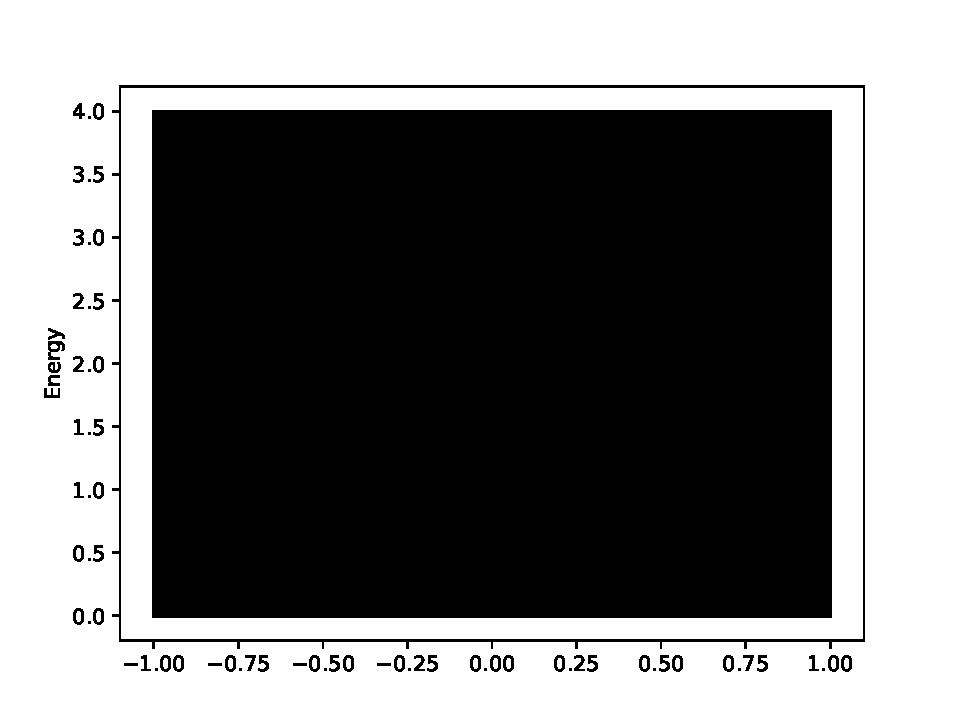
\includegraphics[width=0.8\textwidth]{figs/DOS_HL_normal.pdf}
	\caption{Spectrum of the left lead. Ignore the x-axis tick labels, they do not mean anything. The black bars are eigenenergies.}
\end{figure}
\begin{figure}[!h]
	\centering
	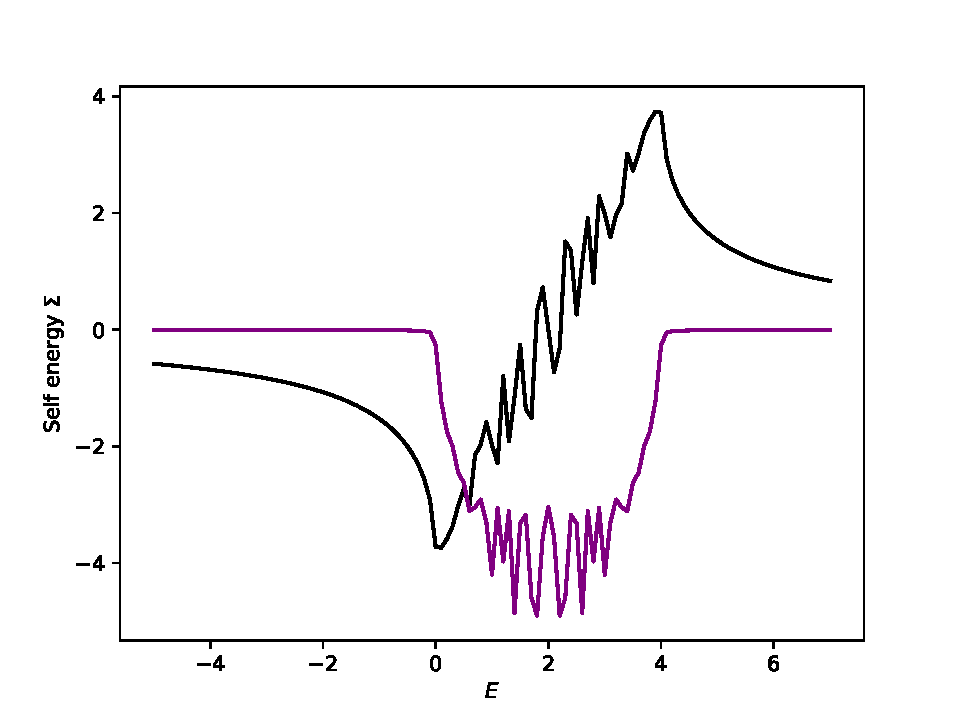
\includegraphics[width=0.8\textwidth]{figs/SelfEnergy_HL_normal.pdf}
	\caption{Selfenergy (\cref{eq:self_energy}). Black: $\mathrm{Re} \Sigma$, purple: $\mathrm{Im} \Sigma$.}
\end{figure}
\begin{figure}[!h]
	\centering
	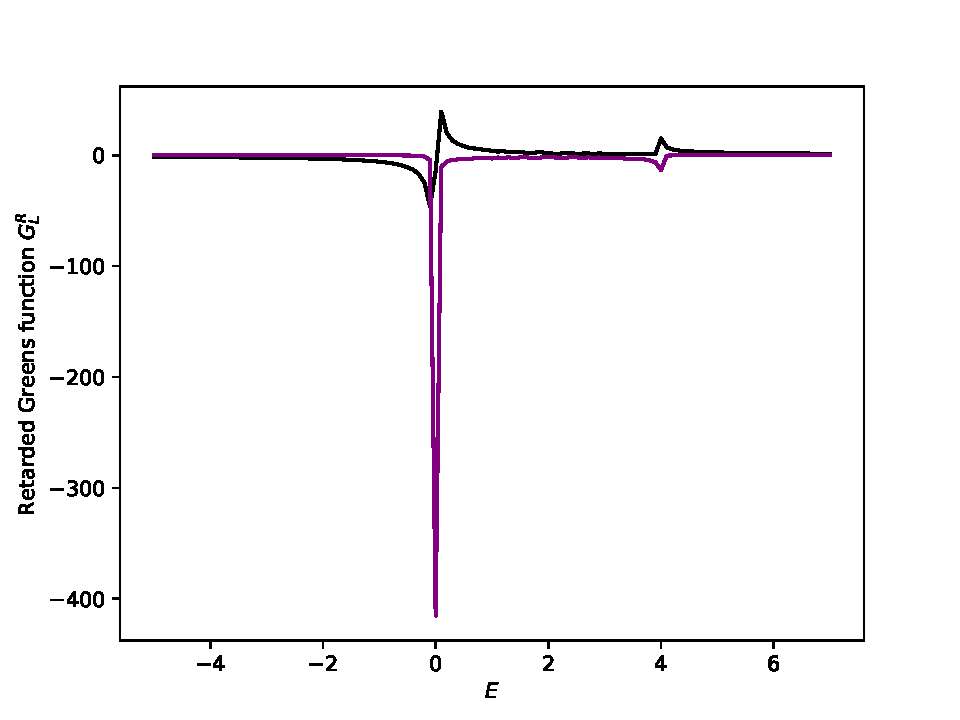
\includegraphics[width=0.8\textwidth]{figs/GreenFunc_HL_normal.pdf}
	\caption{Retarded Greens function (traced) of the left lead. Black: $\mathrm{Re}$, purple: $\mathrm{Im}$.}
\end{figure}
\begin{figure}[!h]
	\centering
	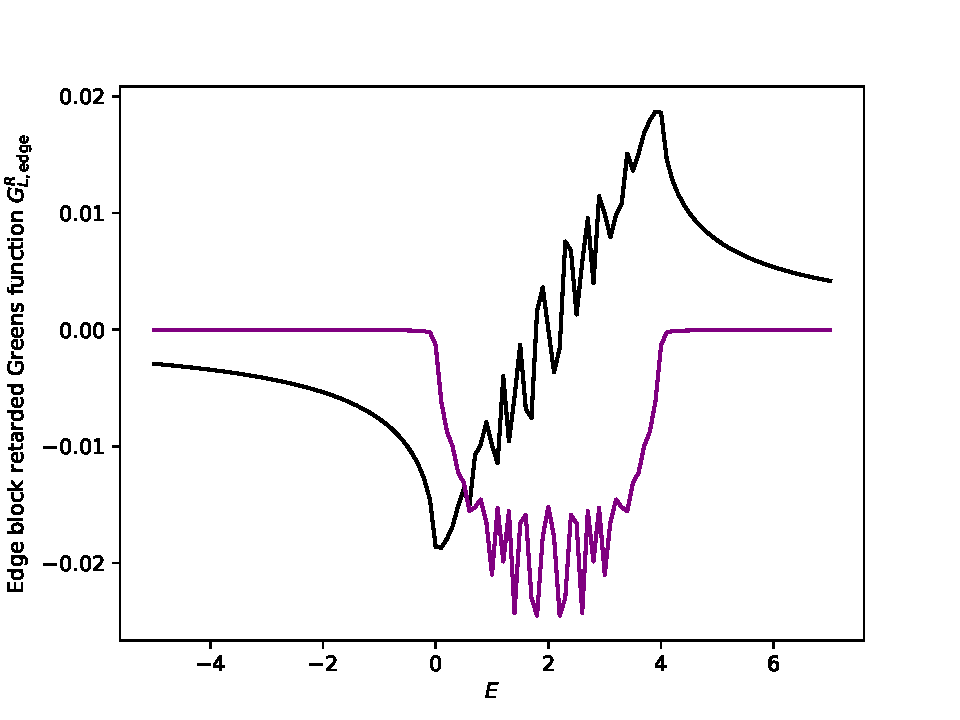
\includegraphics[width=0.8\textwidth]{figs/GreenFunc00_HL_normal.pdf}
	\caption{Retarded Greens function at the edge block of the left lead. Black: $\mathrm{Re}$, purple: $\mathrm{Im}$.}
\end{figure}

\clearpage
\section{Gapped Lead}
\begin{figure}[!h]
	\centering
	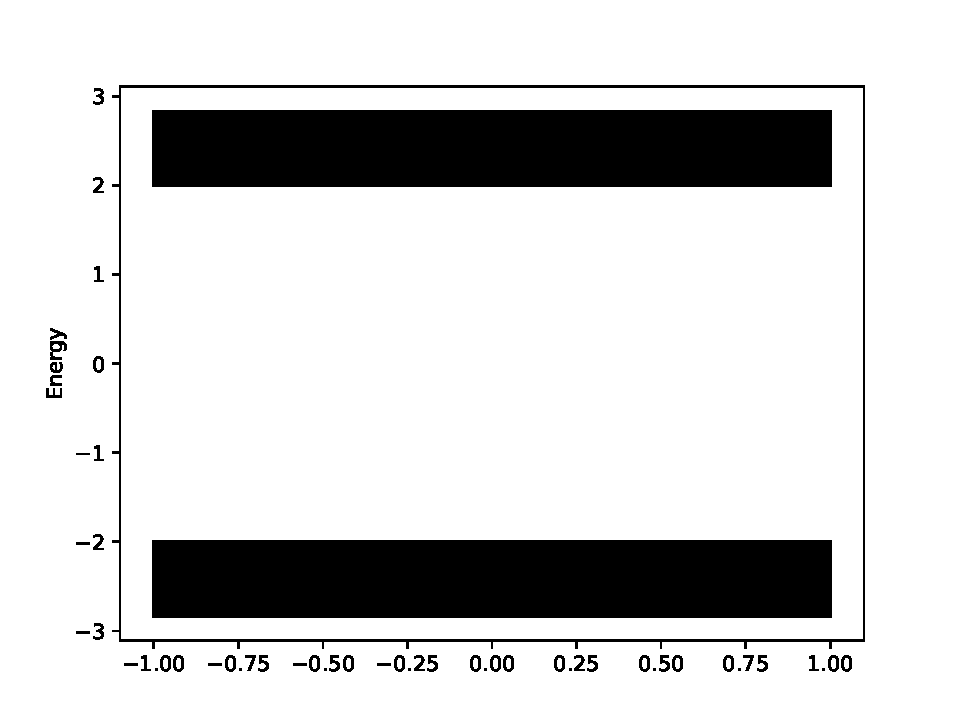
\includegraphics[width=0.8\textwidth]{figs/DOS_HL_gapped.pdf}
	\caption{Spectrum of the left lead. Ignore the x-axis tick labels, they do not mean anything. The black bars are eigenenergies.}
\end{figure}
\begin{figure}[!h]
	\centering
	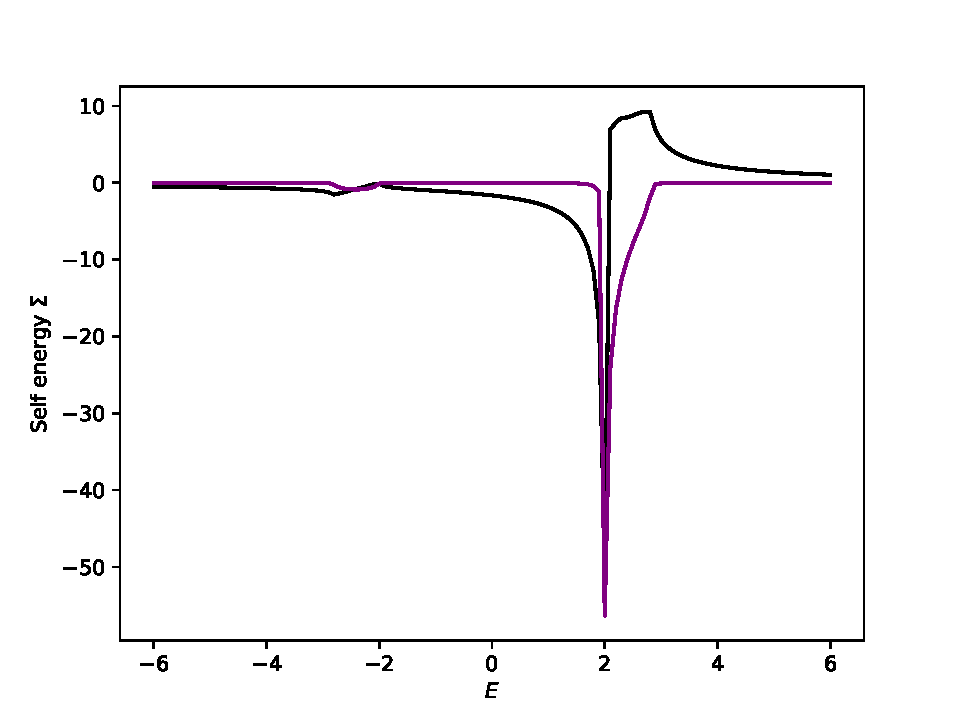
\includegraphics[width=0.8\textwidth]{figs/SelfEnergy_HL_gapped.pdf}
	\caption{Selfenergy (\cref{eq:self_energy}). Black: $\mathrm{Re} \Sigma$, purple: $\mathrm{Im} \Sigma$.}
\end{figure}
\begin{figure}[!h]
	\centering
	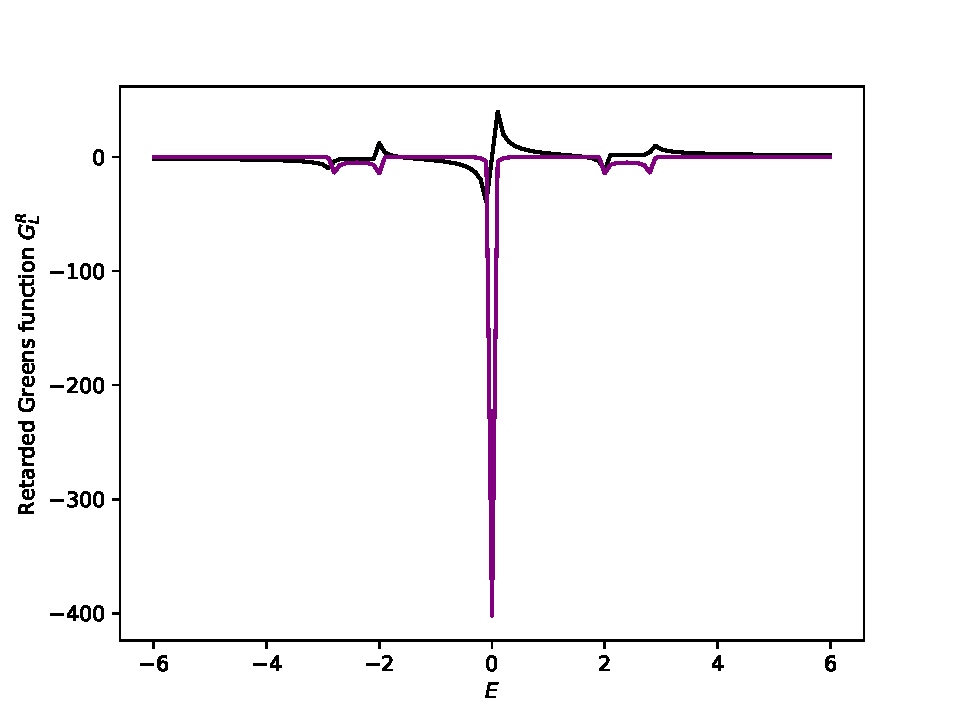
\includegraphics[width=0.8\textwidth]{figs/GreenFunc_HL_gapped.pdf}
	\caption{Retarded Greens function (traced) of the left lead. Black: $\mathrm{Re}$, purple: $\mathrm{Im}$.}
\end{figure}
\begin{figure}[!h]
	\centering
	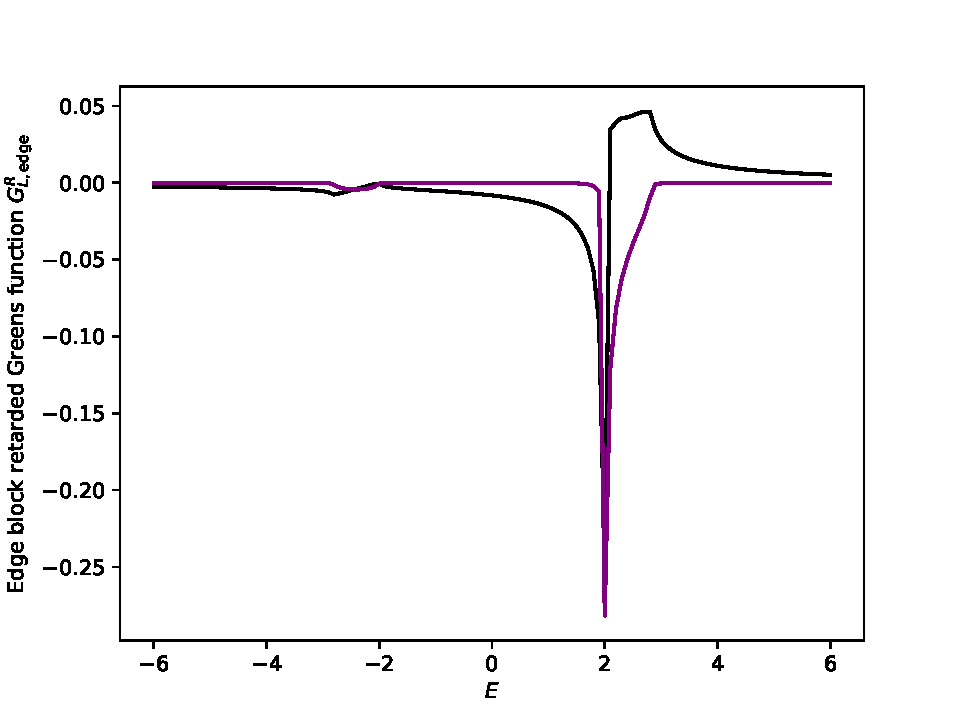
\includegraphics[width=0.8\textwidth]{figs/GreenFunc00_HL_gapped.pdf}
	\caption{Retarded Greens function at the edge block of the left lead. Black: $\mathrm{Re}$, purple: $\mathrm{Im}$.}
\end{figure}
\clearpage
\section{Concluding remarks}
\begin{itemize}
	\item The spectral function is determined (by definition) by the imaginary part of the self energy, which itself is determined entirely by the retarded Greens function at the system-lead edge block. 
	\item As can be seen from the self energy for the gapped case, the imaginary part is zero everywhere in the gap, and non-zero only in the upper and lower band.  
\end{itemize}

\end{document}




